El núcleo del Kit de Desarrollo FX2LP EZ-USB es un CY7C68013A. Dicho circuito integrado, cuya arquitectura se presenta en la Figura \ref{arqEzUSB}, pertenece a la serie FX2LP de la familia de integrados EZ-USB comercializado por Cypress Semiconductors.\\

Esta serie se caracteriza por brindar una conexión USB 2.0 de alta velocidad y bajo consumo energético, especialmente diseñados para productos con autonomía limitada. Se integra un controlador USB completo, incluyendo un transceptor USB, un MIS (Motor de Interfaz Serial), buffers de datos implementados con memorias tipo FIFO (\(First In First Out\); Primero Entrado, Primero Salido), un microcontrolador 8051 mejorado y una interfaz programable hacia los periféricos. Además posee un PLL con divisor configurable a través de los cuales proveen las señales de reloj adecuadas para el correcto funcionamiento del sistema.\\

\begin{figure}[b]
	\centering
	%TODO meter la imagen
	\begin{tikzpicture}[scale=\textwidth/\paperwidth]
		\begin{scope}[
			>=latex,
			node distance=1,
			align=center,
			transform shape
			]
			\node			(aux1)	[]				{};
			\node[core,
			minimum height=95]
			(mis)	[left=of aux1,anchor=north east]	{MIS};
			\node[core]		(ram)	[right=of aux1,anchor=north west, text width=30]	{16 kB RAM};
			\node[perif,
			text width=60]
			(xcvr)	[left=of mis]	{Transceptor USB};
			\node[interior,
			minimum size=60,
			text width=50]
			(uc)	[above=of aux1]	{8051 Mejorado};			
			\node[perif,
			node distance=2.9]
			(pll)	[left=of uc]	{PLL};
			
			\node			(aux2)	[right=of ram.south]{};				
			\node[core,
				text width=120]
							(bus)	[right=of aux2,rotate=90,anchor=north west]	{Bus de datos y direcciones};
			
			\node[perif]	(i2c)	[right=of bus.south east,anchor=north west]	{I2C};
			\node[perif,
				text width=30]
							(gpif)	[right=of bus.south west,anchor=south west] {GPIF};
			\node[perif,
			text width=40]
			(fifo)	[below=of gpif]	{4 kB FIFO};
			\node 			(aux3)	[right=of fifo]	{};
			\node 			(aux5) 	[left=of ram] {};
			
			\draw[<->]	(mis) -- (xcvr);
			\draw[<->]	(ram) -- (ram -| mis.east);
			\draw[<->]	(fifo) -- (fifo -| mis.east);
			\draw[<->]	(ram) to (ram -| bus.north);
			\draw[<->]	(uc) to (uc -| bus.north);
			\draw[<-]	(xcvr) to (xcvr |- pll.south);
			\draw[->]	(pll) to (uc);
			\draw[<->]	(i2c) to (i2c -| bus.south);
			\draw[<->]	(gpif) to (gpif -| bus.south);
			\draw[]		(fifo) -| (aux5.center);
		\end{scope}
		
		\begin{scope}[on background layer]
			\node[contenedor] (fx2) [fit=(pll)(xcvr)(uc)(bus)(mis)(ram)(fifo)(gpif)(i2c)(aux3)]{};
		\end{scope}
		
		\begin{scope}[
			transform shape,
			>=latex
			]
			\node[text width=40,align=center]	(xtal)	[left=of pll]{Xtal \SI{24}{\mega\hertz}};
			\node	(host)	[left=3of xcvr]	{PC};
			\draw[<->,ultra thick] (host) -- node [above,text width=70,midway,align=center]{Comunicación USB} (xcvr);
			\draw[->] (xtal) to (pll);
			\draw[<->,ultra thick] (bus.240) -- node [above,align=center,text width=80] {Datos, direcciones y entradas adicionales}(bus.240 -| fx2.east);
			\draw[<->,thick] (gpif) to (gpif -| fx2.east);
			\draw[<->,thick] (fifo) to (fifo -| fx2.east);
			\draw[<->,thick] (i2c) to (i2c -| fx2.east);
		\end{scope}
	\end{tikzpicture}
%		\includegraphics[width=.7\textwidth]{arqfx2lp.png}
%		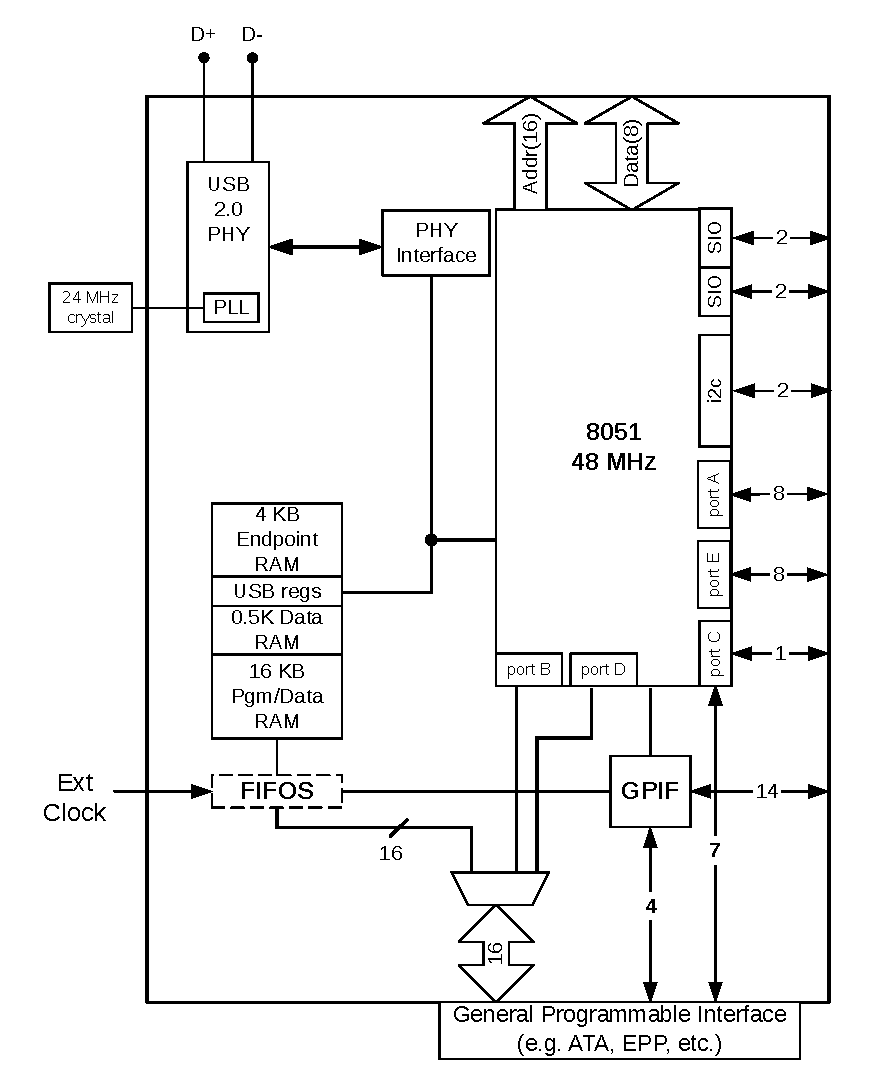
\includegraphics[width=.55\textwidth]{arq.eps}
	%TODO Meter la referencia
	\caption{Arquitectura FX2LP} 
	\label{arqEzUSB}
\end{figure}

De esta forma, se permite al usuario trasmitir datos desde y hacia el anfitrión a través del  mismo puerto USB, o bien via RS-232. Para comunicarse con sistemas periféricos se puede aprovechar el puerto $I^2C$, la interfaz de propósito general, que actúa como maestro y a la cual se le puede acoplar un periférico esclavo, y/o las memorias FIFO en modo esclavo que puede ser conectada a un sistema maestro. Esto brinda muchas alternativas, desde la conexión a puertos estandar, como ser ATA, PCMCIA, EPP, etc. o también la conexión de dispositivos tales como DSP's y FPGA's.\\

Este trabajo utiliza particularmente las memorias FIFO en modo esclavo, que responden a las diferentes señales que les proporciona un maestro externo implementado con un FPGA; por lo que a continuación se explicitan algunos detalles referidos a ellos, con lo que se busca aclarar el funcionamiento y que el lector comprenda los fundamentos de las configuraciones que se plasmarán en el código del firmware.\\

\subsection{Motor de Interfaz Serial}

	La comunicación USB entre el controlador FX2LP y la PC se realiza a través del transceptor, unido al MIS. Como se observa en la Figura \ref{usbxcvr}, el usuario, a fin de intercambiar datos, solo debe colocar o extraer los datos de registros destinados a tal fin y modificar las banderas de handshaking, que en la figura se observan como ACK (abreviación del ingles {\it acknowledge}, que significa reconocer, aceptar o agradecer), que indican si el sistema está disponible, si los datos fueron colocados o leídos, dependiendo el caso tratado. De forma automática, el MIS y el transceptor USB se encargan de empaquetar, enviar, recibir y desempaquetar toda la información, así como leer los tokens que emite el host, calcular y corroborar los códigos cíclicos de detección de errores y todo lo relacionado al protocolo propiamente dicho.\\

	\begin{figure}[ht]
		\centering
		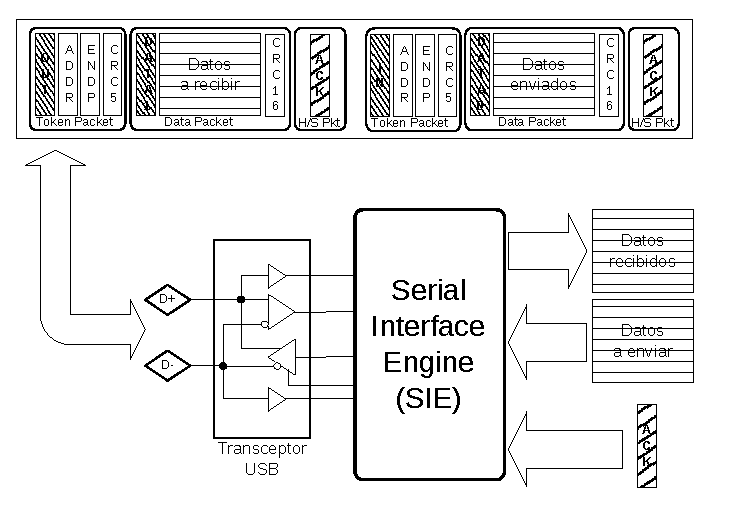
\includegraphics[width=.8\textwidth]{usbxcvr}
		\caption{Implementación del enlace USB realizado por el EZ-USB}
		\label{usbxcvr}
	\end{figure}
		
\subsection{Buffers de extremos}
	El MIS guarda los datos que aún no han sido enviados y/o los que han sido recibidos pero no leídos por ningún periférico en una memoria RAM específica, denominada buffer de extremo.\\
	
	La norma USB define a un dispositivo extremo como una porción exclusiva e identificable de un dispositivo USB que es fuente o un sumidero de información. En otras palabras, USB ve a cada extremo como una memoria FIFO de donde surge o finalizan la información. En ingles, el termino extremo se escribe endpoint, por lo que, en adelante, cuando se hable de ellos se abreviara como EP o EPx, siendo la x un número que indica la dirección del extremo.\\
	
	La serie de controladores FX2LP dispone de hasta 7 EP's programables, los cuales deben poseer al menos dos buffers.\\
	
	La norma USB indica que cualquier dispositivo USB debe poseer un EP con dirección 0 que se destina para control y configuración, por lo que el controlador está dotado de \SI{64}{\byte} para este fin. Es el único EP que puede ser bidireccional en el sentido del flujo de datos. A través de él, anfitrión y dispositivo intercambiarán solo transferencias de control.\\
	
	Luego, se incorpora un EP1, que posee dos buffers fijos, o sea no configurables, de 64 bytes, uno como entrada y el otro como salida.\\
	
	\begin{figure}[t]
		\centering
		\begin{tikzpicture}[scale=.7*\textwidth/\paperwidth,node distance=2.7]
			\begin{scope}[transform shape]
				\begin{scope}[node distance=0.4]
					\node[buf]	(ep2b1)	[anchor=north]		{\ep{1}{2}{512}};
					\node[buf]	(ep2b2)	[below=of ep2b1]	{\ep{2}{2}{512}};
					\node[obuf]	(ep4b1) [below=of ep2b2]	{\ep{1}{4}{512}};
					\node[buf]	(ep4b2) [below=of ep4b1]	{\ep{2}{4}{512}};
					\node[obuf]	(ep6b1)	[below=of ep4b2]	{\ep{1}{6}{512}};
					\node[buf]	(ep6b2)	[below=of ep6b1]	{\ep{2}{6}{512}};
					\node[obuf]	(ep8b1)	[below=of ep6b2]	{\ep{1}{8}{512}};
					\node[buf]	(ep8b2)	[below=of ep8b1]	{\ep{2}{8}{512}};
				\end{scope}
				
				\begin{scope}[node distance=0.4, xshift=90]
					\node[buf]	(ep2b3)	[anchor=north]		{\epg{1}{2}{1024}};
					\node[obuf] (ep2b4)	[below=of ep2b3]	{\epg{2}{2}{1024}};
					\node[obuf]	(ep2b5)	[below=of ep2b4]	{\epg{3}{2}{1024}};
					\node[obuf]	(ep8b3)	[below=of ep2b5]	{\ep{1}{8}{512}};
					\node[buf]	(ep8b4)	[below=of ep8b3]	{\ep{2}{8}{512}};
				\end{scope}
			\end{scope}
		
			\begin{scope}[on background layer]
				rounded corners,]
				\node[env, fit=(ep2b1)(ep2b2)]			(ep21)	{};
				\node[env, fit=(ep4b1)(ep4b2)]			(ep41)	{};
				\node[env, fit=(ep6b1)(ep6b2)]			(ep61)	{};
				\node[env, fit=(ep8b1)(ep8b2)]			(ep81)	{};
				\node[env, fit=(ep2b3)(ep2b4)(ep2b5)]	(ep22)	{};
				\node[env, fit=(ep8b3)(ep8b4)]			(ep82)	{};
				\node[draw=black,fit=(ep21)(ep82)](marco){};
			\end{scope}
		
			\begin{scope}[transform shape]
				\draw (marco.north) to (marco.south);
				\node[left=of ep2b1.north east,anchor=north east](add1)	{0xF000};
				\node[left=of ep2b1.south east,anchor=south east](add2)	{0xF1FF};
				\node[left=of ep2b2.north east,anchor=north east](add3)	{0xF200};
				\node[left=of ep4b1.north east,anchor=north east](add4)	{0xF400};
				\node[left=of ep6b1.north east,anchor=north east](add5)	{0xF800};
				\node[left=of ep8b1.north east,anchor=north east](add6)	{0xFC00};
				\node[left=of ep8b2.south east,anchor=south east](add7)	{0xFFFF};
				\draw[dashed] (add1.north west) to (add1.north west -| marco.east);
				\draw[dashed] (add3.north west) to (add3.north west -| ep21.east);
				\draw[dashed] (add4.north west) to (add4.north west -| marco.east);
				\draw[dashed] (add5.north west) to (add5.north west -| marco.east);
				\draw[dashed] (add6.north west) to (add6.north west -| marco.east);
				\draw[dashed] (add7.south west) to (add7.south west -| marco.east);
			\end{scope}
	\end{tikzpicture}
	\caption{Buffers de extremos con sus direcciones de memoria. El cuadro de la izquierda muestra la configuración por defecto. El derecho, la implementada en este trabajo.}
	\label{epbuf}
	\end{figure}
	
	Finalmente, \SI{4}{\kibi\byte} de memoria debe ser configurada para los EP2, EP4, EP6 y EP8. La configuración de los EP la realiza el firmware en tiempo de ejecución. Las variables, conforme a los requerimientos de ancho de banda, acceso al bus son:
	
	\begin{itemize}
		\item Tamaño: Dependiendo del extremo a configurar puede ser de 512 o 1024 bytes.
		\item Tipo de acceso al bus: Definido según la norma USB, este tipo puede ser por bultos, isocrónico o de interrupción.
		\item Cantidad de buffers: Dependiendo del extremo, puede ser dos, tres o cuatro buffers por extremo.
		\item Habilitación: Se debe indicar al sistema si los extremos se usan o no. El EP no valido, no responderá a un pedido de entrada o salida.
	\end{itemize}
	
	La Figura \ref{epbuf} muestra solo dos las posibles configuraciones de los extremos. A la izquierda se observa la configuración por defecto del controlador FX2LP. Esto es, los cuatro EP's habilitados, con 512 bytes cada uno, buffers dobles y comunicación por bultos. A la derecha se muestra la configuración elegida para este trabajo, es decir, solo son válidos el EP2 y EP8. EP2 posee tres buffers de 1024 bytes y el EP8 dos buffers con 512 bytes de capacidad cada uno. Siempre hay que considerar no se dispone más que \SI{4}{\kibi\byte} de memoria\\
	
	La característica de los buffers múltiples evita la congestión de datos. Con doble buffer, un periférico (o el microcontrolador) coloca o extrae datos de un buffer, mientras otro, del mismo EP, se encuentra enviando o recibiendo datos mediante el MIS. Cuando se configura un triple buffer, se agrega una porción mas de memoria a la reserva. De esta forma, se le otorga al sistema una gran capacidad de datos y ancho de banda.\\
	
	Un detalle importante de los buffers múltiples es que, a la vista del controlador y/o de un periférico, el buffer posee una sola y única dirección y, es el sistema mismo quien se encarga de seleccionar el buffer en uso. Esto quiere decir que, por ejemplo, teniendo 4 buffers de 512 bytes cada uno, el 8051 verá solo uno de 512 bytes, sin necesidad de identificar con cuál de los cuatro está trabajando.\\   

\subsection{Memorias FIFO esclavas}		

	Desde un punto de vista digital, el MIS recibe y envía datos desde y hacia el puerto USB. Para ello utiliza un cristal de \SI{24}{\mega\hertz}. Por su parte, un sistema externo puede o no proveer una señal de reloj y manejo de datos propio. El controlador USB incorpora memorias FIFO que se encargan de proveer una interfaz entre el MIS y un dispositivo externo, salvando el problema de poseer dos relojes diferentes e independientes.\\
	
	Estas memorias funcionan en modo esclavo, es decir, se debe conectar, al controlador, un dispositivo  capaz de proveer una lógica maestra externa que comande la entrada y salida de datos desde una memoria FIFO hacia o desde el exterior.\\
	
	Para los fines del presente trabajo, este modo de funcionamiento es óptimo, ya que dotando al FPGA de una máquina de estados mínima, se logra la transferencia de datos en los tiempos requeridos.\\
	
	El sistema de bus permite conectar a estas memorias hasta cuatro dispositivos diferentes. Por esto, existe una memoria FIFO para cada uno de los EP programables en el buffer de extremos.\\
	
	\begin{figure}[ht]
		\centering
		\begin{tikzpicture}[scale=1*\textwidth/\paperwidth]
			\begin{scope}[transform shape,node distance=4,>=latex]
				\node[simple]	(fifo)		[]	 			{FIFO's Esclavas};
				\node[simple]	(master)	[right=of fifo]	{Maestro Externo};
				\draw[<->,thick]	([yshift=5*110/6]fifo.east) --node [above]{IFCLK} ([yshift=5*110/6]master.west);
				\draw[<->,thick]	([yshift=4*110/6]fifo.east) --node [above]{FD[15:0]} ([yshift=4*110/6]master.west);
				\draw[<-,thick]	([yshift=3*110/6]fifo.east) --node [above]{FIFOADR[1:0]} ([yshift=3*110/6]master.west);
				\draw[->,thick]	([yshift=2*110/6]fifo.east) --node [above]{FLAGA} ([yshift=2*110/6]master.west);
				\draw[->,thick]	([yshift=1*110/6]fifo.east) --node [above]{FLAGB} ([yshift=1*110/6]master.west);
				\draw[->,thick]	([yshift=0*110/6]fifo.east) --node [above]{FLAGC} ([yshift=0*110/6]master.west);
				\draw[->,thick]	([yshift=-1*110/6]fifo.east) --node [above]{FLAGD} ([yshift=-1*110/6]master.west);
				\draw[<-,thick]	([yshift=-2*110/6]fifo.east) --node [above]{SLOE} ([yshift=-2*110/6]master.west);
				\draw[<-,thick]	([yshift=-3*110/6]fifo.east) --node [above]{SLWR} ([yshift=-3*110/6]master.west);
				\draw[<-,thick]	([yshift=-4*110/6]fifo.east) --node [above]{SLRD} ([yshift=-4*110/6]master.west);
				\draw[<-,thick]	([yshift=-5*110/6]fifo.east) --node [above]{PKTEND} ([yshift=-5*110/6]master.west);
			\end{scope}				
		\end{tikzpicture}
		\caption{Configuración de puertos para la interfaz entre las FIFO's y un maestro externo}
		\label{interfazfifo}
	\end{figure}

	La Figura \ref{interfazfifo} muestra la interfaz entre las memorias FIFO's y un maestro esclavo. Estos son:
	
	\begin{itemize}
		\item IFCLK: señal de reloj. En caso de conectar las memorias en modo asincrónico, no es necesario. La señal de reloj puede ser establecida por el controlador o por el dispositivo de control en forma programable.
		\item FD[15:0]: constituye el bus de datos. Según se programe, este puede ser de 8 o 16 bits.
		\item FIFOADDR[1:0]: puerto de direcciones. A través de el se selecciona la memoria activa en el bus.
		\item FLAGx: Los cuatro puertos de flag son configurables e indican memoria llena, vacía o un nivel programable, en forma fija sobre una memoria en particular o que indiquen sobre la memoria activa.
		\item SLOE, SLWR, SLRD: son las señales de control. A través de ellas el maestro entrega las ordenes de lectura y escritura.
		\item PKTEND: a través de este puerto el maestro indica que terminó una transferencia de datos.
	\end{itemize}

\subsection{Modos de entrada y salida automáticos}
	\begin{figure}[ht]
		\centering
		\begin{tikzpicture}[scale=0.8\textwidth/\paperwidth,text width=5em,align=center,>=latex,node distance=31mm]		
		\begin{scope}[transform shape]
		\node[interior]	(mis)									{MIS};
		\node			(im)	[right=of mis]					{};
		\node[interior]	(uc)	[above=of im]					{$\mu$C};
		\node[interior] (fifo)	[right=of im,text width=4em]	{FIFOs Esclavas};
		\node			(et)	[left=of uc]					{FX2LP};
		
		\draw[->]([xshift=1.5mm]fifo.north)to node[above,mode text]{MODO ENTRADA MANUAL} ([yshift=1mm]uc.east);
		\draw[->]([yshift=1mm]uc.west)to node[above,mode text]{MODO ENTRADA MANUAL}([xshift=-1.5mm]mis.north);
		\draw[->] ([yshift=-1mm]uc.east)to node[below,mode text]{MODO SALIDA MANUAL}([xshift=-1.5mm]fifo.north);
		\draw[->]([xshift=1.5mm]mis.north)to node[below,mode text]{MODO SALIDA MANUAL}([yshift=-1mm]uc.west);
		
		\draw[->]([yshift=1mm]fifo.west)to node[above,mode text]{MODO AUTO ENTRADA}([yshift=1mm]mis.east);
		\draw[->]([yshift=-1mm]mis.east)to node[below,mode text]{MODO AUTO SALIDA}([yshift=-1mm]fifo.west);
		
		\node[exterior]	(pc)	[left=of mis]	{Host};
		\draw[->]([yshift=1mm]mis.west)to([yshift=1mm]pc.east);
		\draw[->]([yshift=-1mm]pc.east)to([yshift=-1mm]mis.west);
		
		\node[exterior]	(fpga)	[right=of fifo]	{Maestro Externo};
		\draw[->]([yshift=1mm]fifo.east)to node[above]{Banderas}([yshift=1mm]fpga.west);
		\draw[<-]([yshift=-1mm]fifo.east)to node[below]{Control}([yshift=-1mm]fpga.west);
		\end{scope}	
		
		\begin{scope}[on background layer]
		\node(fx)[rounded corners,fill=black!10,fit=(mis)(uc)(fifo)(et)]{};
		\end{scope}
		\end{tikzpicture}
		\caption{Modos de conexión de la memoria FIFO, el microntrolador y el MIS}
		\label{modesfifo}
	\end{figure}

	
	Los datos que se reciben o envían a través del MIS. Pueden ser enviados en forma automática desde y hacia las memorias FIFO, o bien, pueden ser dirigidos a través del microcontrolador. Esto último permite leer, modificar, suprimir, agregar y/o generar nuevos datos antes de ser remitidos como paquete, es decir, todos juntos, a su respectivo EP. Estos caminos se pueden ver en la Figura \ref{modesfifo}.\\
	
	Los fabricantes llaman a estos caminos "MODO MANUAL", en caso de enviar los datos a través del 8051, y "MODO AUTOMÁTICO", cuando la comunicación es directa entre el MIS y las FIFO. Además, se programan en forma independiente para cada extremo, sea este de salida o entrada.\\
	
	Se debe notar en la Figura \ref{modesfifo} que se refiere a paquetes de entrada cuando estos poseen una dirección que se inicia en un periférico y termina en el anfitrión y de salida cuando llevan el sentido contrario. Esto se debe al carácter {\it anfritión-céntrico} de la comunicación USB, en donde el principal componente es el anfitrión y a él se acoplan los diferentes dispositivos.\\
	
	